\documentclass[11pt,a4paper]{article}
\usepackage[margin=20mm]{geometry}
\usepackage[T1]{fontenc}
\usepackage{lmodern}
\usepackage{amsmath,amssymb,booktabs,tabularx,array,tikz,graphicx}
\usepackage[hidelinks]{hyperref}
\usepackage{enumitem}
\setlist[itemize]{leftmargin=*,itemsep=3pt,topsep=4pt}
\setlength{\parindent}{0pt}
\setlength{\parskip}{5pt}
\renewcommand{\arraystretch}{1.2}
\newcommand{\state}[1]{\textsf{#1}}
\newcommand{\LN}{\operatorname{LN}}
\newcommand{\GELU}{\operatorname{GELU}}
\begin{document}
\begin{center}
{\LARGE\bfseries BCJRFormer ASIC Architecture}\par
\vspace{3pt}
{\large Design Review}\par
Taimor Sabek and Haiel Bader
\end{center}

\section*{1\quad Scope and architecture}
We propose a sequential ASIC implementation of the BCJRFormer inference core.
We start with prepared window features* and a padding mask and produce decoded-position logits*.


We have 5 stages, each with a separate controller. each one of them represents a block in the diagram of the transformer architecture.
The stages are: input embedding, position and read embedding, encoder layers, final projection and read aggregation. 
Each stage executes in order; the next stage starts only after the previous stage's output writes have committed. 
The padding mask is retained for the whole frame. 
A separate parameter memory (ROM) supplies learned weights, biases, embedding tables and normalization parameters.

\begin{center}
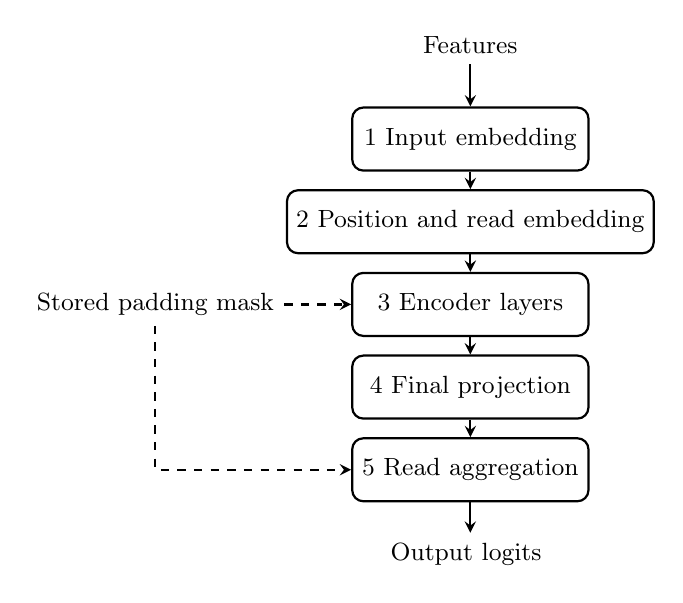
\begin{tikzpicture}[>=stealth,thick,every node/.style={font=\small,align=center}]
\node[draw,rounded corners,minimum width=3cm,minimum height=8mm] (a) at (0,0) {1 Input embedding};
\node[draw,rounded corners,minimum width=3cm,minimum height=8mm] (b) at (0,-1.05) {2 Position and read embedding};
\node[draw,rounded corners,minimum width=3cm,minimum height=8mm] (c) at (0,-2.10) {3 Encoder layers};
\node[draw,rounded corners,minimum width=3cm,minimum height=8mm] (d) at (0,-3.15) {4 Final projection};
\node[draw,rounded corners,minimum width=3cm,minimum height=8mm] (e) at (0,-4.20) {5 Read aggregation};
\draw[->] (a)--(b) node[midway,right] {};
\draw[->] (b)--(c) node[midway,right] {};
\draw[->] (c)--(d) node[midway,right] {};
\draw[->] (d)--(e) node[midway,right] {};
\draw[->] (0,.95)--(a) node[pos=0,above] {Features};
\draw[->] (e)--(0,-5) node[below] {Output logits };
\node (mask) at (-4,-2.1) {Stored padding mask};
\draw[->,dashed] (mask)--(c);
\draw[->,dashed] (mask.south)--(-4,-4.2)--(e.west);
\end{tikzpicture}
\end{center}


\textbf{Frame control} A frame contains the noisy reads of one encoded sequence. $N$ is the number of target bit positions in that sequence. Load features and mask, run stages 1--5, transfer the $N$ logits, then report completion. Parameters must be available before accepting a frame and remain available across frames. The ASIC holds each output until the receiver accepts it, then advances to the next output.


\textbf{* Window features:} For each target position in each noisy read, preprocessing builds a small table of numbers showing how well nearby received locations and possible bit patterns match that position. These tables are stored in the input tensor \texttt{y} before entering the ASIC.

\textbf{* Logits:} Output scores indicating whether each decoded bit is more likely to be 0 or 1. A positive score favors 1; a negative score favors 0. They are scores, not probabilities or percentages.




\newpage
\section*{Frame input and overall control}
\textbf{Input:} prepared window features and their padding mask for one encoded sequence. The mask marks padded positions, not the value of the decoded bits. The trained weights must already be available in parameter memory.

\textbf{Output:} $N$ logits, one per target bit position, followed by completion status.

\textbf{FSM} means finite-state machine: circles are controller states and arrows show the order of work. This controller starts the five stage controllers in sequence; the stage-specific FSMs are placed inside their own sections below.
\begin{center}
\resizebox{\textwidth}{!}{%
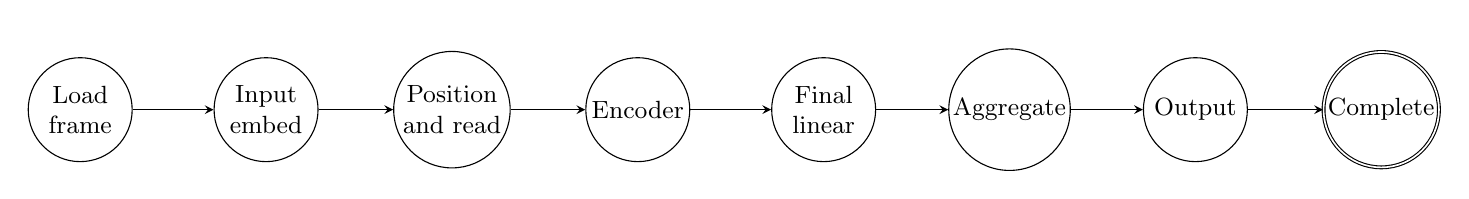
\begin{tikzpicture}[x=0.02cm,y=-0.02cm,>=stealth,every node/.style={font=\small,align=center}]
\node[draw,circle,minimum size=1.32cm,inner sep=1pt] (n0) at (45,85) {Load\\frame};
\node[draw,circle,minimum size=1.32cm,inner sep=1pt] (n1) at (163,85) {Input\\embed};
\node[draw,circle,minimum size=1.32cm,inner sep=1pt] (n2) at (281,85) {Position\\and read};
\node[draw,circle,minimum size=1.32cm,inner sep=1pt] (n3) at (399,85) {Encoder};
\node[draw,circle,minimum size=1.32cm,inner sep=1pt] (n4) at (517,85) {Final\\linear};
\node[draw,circle,minimum size=1.32cm,inner sep=1pt] (n5) at (635,85) {Aggregate};
\node[draw,circle,minimum size=1.32cm,inner sep=1pt] (n6) at (753,85) {Output};
\node[draw,circle,minimum size=1.32cm,inner sep=1pt,double] (n7) at (871,85) {Complete};
\draw[->] (n0) -- node[above=8mm,font=\scriptsize]{} (n1);
\draw[->] (n1) -- node[above=8mm,font=\scriptsize]{} (n2);
\draw[->] (n2) -- node[above=8mm,font=\scriptsize]{} (n3);
\draw[->] (n3) -- node[above=8mm,font=\scriptsize]{} (n4);
\draw[->] (n4) -- node[above=8mm,font=\scriptsize]{} (n5);
\draw[->] (n5) -- node[above=8mm,font=\scriptsize]{} (n6);
\draw[->] (n6) -- node[above=8mm,font=\scriptsize]{} (n7);
\end{tikzpicture}}
\end{center}
Load the full frame and save its mask. Start Stage 1 and wait until its results are stored; do the same for Stages 2--5. Output transfers one stored logit at a time and waits whenever the receiver is not ready. Complete is reached only after the final accepted transfer.

For every FSM below, an operation is started once and its state waits until the operation finishes. Memory-read states include waiting for the returned value. A write is finished only when the memory confirms it. Counters advance only after the associated operation finishes. Completion remains available until accepted; then the controller returns to idle. Fatal hardware errors stop new work, allow already accepted operations to finish and require reset before retry. An empty position in Stage 5 is instead a recoverable frame error: discard the frame and return to idle after its error status is accepted, without reset.

\newpage
\section*{2\quad Stage 1: Input embedding}
\subsection*{Purpose, definitions, input and output}
This stage turns the window for each position in each read into the representation used by the transformer. A \textbf{token} means one target position in one read, not a whole read.
\begin{itemize}
\item $B=1$: one frame at a time. A frame contains the noisy reads of one encoded sequence.
\item $M$: number of read slots, including unused slots filled with padding.
\item $N$: target bit positions in the encoded sequence, not the length of a noisy received read.
\item $W$: number of nearby received locations considered in one window.
\item $S$: number of candidate bit patterns represented at each window location.
\item $F=WS$: number of input numbers in one window. These are the window features.
\item $L=MN$: total number of tokens (read-position pairs), including padded tokens.
\item $D$: number of output numbers used to represent each token. This is the configured model width, called \texttt{d\_model} in Python.
\item $m,n,t$: read, position and token indices, starting at zero; $t=mN+n$, with $0\leq t<L$.
\end{itemize}
These sizes are not learned weights. $L$ and $F$ are calculated from the selected input sizes; $D$ comes from the model configuration.

\textbf{Input:} prepared window features in \texttt{y}, with shape $[B,M,N,W,S]$. For one read and position, its $W\times S$ table contains $F$ numbers. We call those same numbers $x_t[f]$, where $0\leq f<F$; this changes their indexing, not their values. $[L,F]$ means $L$ tokens with $F$ numbers each.

\textbf{Output:} $e[L,D]$, meaning $L$ tokens with $D$ numbers each, sent to Stage 2. The padding mask marks unused read positions and is saved unchanged for Stages 3 and 5.

\subsection*{FSM and stage control}
An \textbf{FSM (finite-state machine)} is the controller that moves between the steps shown by circles. Each arrow is taken only after the current operation finishes. A state may take many clock cycles. A double circle means completion, held until accepted by the receiving controller.
\begin{center}
\resizebox{\textwidth}{!}{%
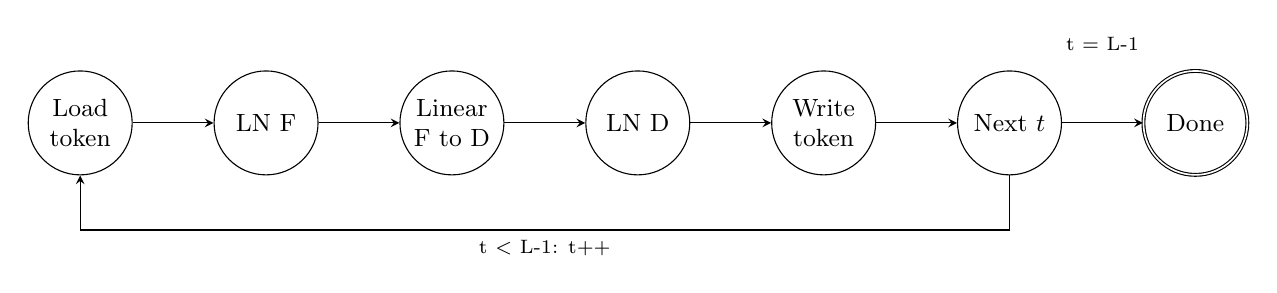
\begin{tikzpicture}[x=0.02cm,y=-0.02cm,>=stealth,every node/.style={font=\small,align=center}]
\node[draw,circle,minimum size=1.32cm,inner sep=1pt] (n0) at (45,85) {Load\\token};
\node[draw,circle,minimum size=1.32cm,inner sep=1pt] (n1) at (163,85) {LN F};
\node[draw,circle,minimum size=1.32cm,inner sep=1pt] (n2) at (281,85) {Linear\\F to D};
\node[draw,circle,minimum size=1.32cm,inner sep=1pt] (n3) at (399,85) {LN D};
\node[draw,circle,minimum size=1.32cm,inner sep=1pt] (n4) at (517,85) {Write\\token};
\node[draw,circle,minimum size=1.32cm,inner sep=1pt] (n5) at (635,85) {Next $t$};
\node[draw,circle,minimum size=1.32cm,inner sep=1pt,double] (n6) at (753,85) {Done};
\draw[->] (n0) -- node[above=8mm,font=\scriptsize]{} (n1);
\draw[->] (n1) -- node[above=8mm,font=\scriptsize]{} (n2);
\draw[->] (n2) -- node[above=8mm,font=\scriptsize]{} (n3);
\draw[->] (n3) -- node[above=8mm,font=\scriptsize]{} (n4);
\draw[->] (n4) -- node[above=8mm,font=\scriptsize]{} (n5);
\draw[->] (n5) -- node[above=8mm,font=\scriptsize]{t = L-1} (n6);
\draw[->] (n5.south) -- (635,153) -- node[below,font=\scriptsize]{t $<$ L-1: t++} (45,153) -- (n0.south);
\end{tikzpicture}}
\end{center}
Start with $t=0$. Load its $F$ window numbers, normalize them, run the $F$-to-$D$ linear calculation, normalize the $D$ results, and store them. After all $D$ writes finish, advance to the next token. Stage 2 starts only after all $L$ tokens are stored. Padded tokens also pass through these calculations.

\subsection*{Internal blocks and math}
\[
u_t=\LN_F(x_t),\qquad v_t=W^{emb}u_t+b^{emb},\qquad e_t=\LN_D(v_t).
\]
$u_t$ contains $F$ normalized inputs; $v_t$ contains $D$ linear results; $e_t$ contains $D$ normalized outputs. $\LN$ means layer normalization, defined below. $W^{emb}[D,F]$ is the learned weight table and $b^{emb}[D]$ is the learned bias (a constant added to each output). The superscript $emb$ labels embedding parameters; it is not a power.

\subsection*{Blocks 1 and 3: Layer normalization}
For an input vector $a$ containing $J$ numbers:
\[
\mu=\frac1J\sum_{j=0}^{J-1}a_j,\qquad
v=\frac1J\sum_{j=0}^{J-1}(a_j-\mu)^2,\qquad
o_j=\gamma_j\frac{a_j-\mu}{\sqrt{v+\epsilon}}+\beta_j.
\]
$J=F$ in block 1 and $J=D$ in block 3. $j$ selects a number; $\mu$ is the mean; $v$ is the variance (mean squared distance from the mean). $\epsilon=10^{-5}$ prevents division by zero. $\gamma_j,\beta_j$ are learned scale and offset values; $o_j$ is the output. The two blocks have separate learned values.
\begin{center}
\resizebox{\textwidth}{!}{%
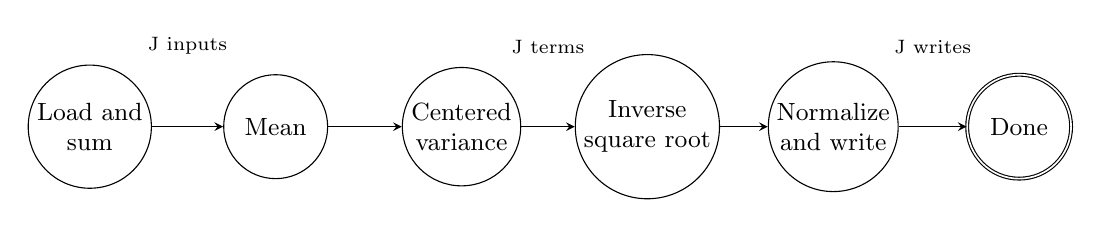
\begin{tikzpicture}[x=0.02cm,y=-0.02cm,>=stealth,every node/.style={font=\small,align=center}]
\node[draw,circle,minimum size=1.32cm,inner sep=1pt] (n0) at (45,85) {Load and\\sum};
\node[draw,circle,minimum size=1.32cm,inner sep=1pt] (n1) at (163,85) {Mean};
\node[draw,circle,minimum size=1.32cm,inner sep=1pt] (n2) at (281,85) {Centered\\variance};
\node[draw,circle,minimum size=1.32cm,inner sep=1pt] (n3) at (399,85) {Inverse\\square root};
\node[draw,circle,minimum size=1.32cm,inner sep=1pt] (n4) at (517,85) {Normalize\\and write};
\node[draw,circle,minimum size=1.32cm,inner sep=1pt,double] (n5) at (635,85) {Done};
\draw[->] (n0) -- node[above=8mm,font=\scriptsize]{J inputs} (n1);
\draw[->] (n1) -- node[above=8mm,font=\scriptsize]{} (n2);
\draw[->] (n2) -- node[above=8mm,font=\scriptsize]{J terms} (n3);
\draw[->] (n3) -- node[above=8mm,font=\scriptsize]{} (n4);
\draw[->] (n4) -- node[above=8mm,font=\scriptsize]{J writes} (n5);
\end{tikzpicture}}
\end{center}
Sum the $J$ inputs; divide by $J$; sum their squared differences from the mean and divide by $J$; compute $1/\sqrt{v+\epsilon}$; then calculate and store each $o_j$. Recalculate mean and variance for every token. Keep the inputs until all passes finish.

\subsection*{Block 2: Linear calculation}
\[
v_t[j]=b^{emb}_j+\sum_{f=0}^{F-1}W^{emb}_{j,f}u_t[f],\qquad 0\leq j<D.
\]
Each output is a weighted sum of all $F$ inputs plus its bias. Keep the input vector in separate storage until all $D$ outputs are calculated.

\textbf{Linear FSM:} here $I=F$ is the input count and $O=D$ is the output count. In this diagram $O$ is a count, not the attention output in Stage 3.
\begin{center}
\resizebox{\textwidth}{!}{%
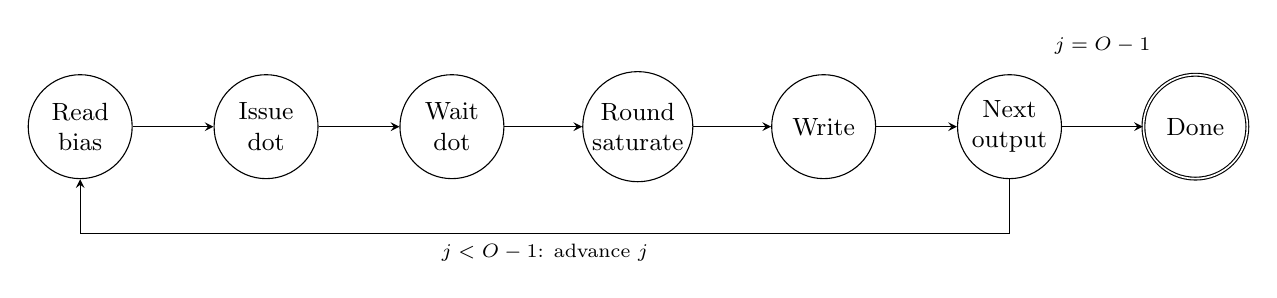
\begin{tikzpicture}[x=0.02cm,y=-0.02cm,>=stealth,every node/.style={font=\small,align=center}]
\node[draw,circle,minimum size=1.32cm,inner sep=1pt] (n0) at (45,85) {Read\\bias};
\node[draw,circle,minimum size=1.32cm,inner sep=1pt] (n1) at (163,85) {Issue\\dot};
\node[draw,circle,minimum size=1.32cm,inner sep=1pt] (n2) at (281,85) {Wait\\dot};
\node[draw,circle,minimum size=1.32cm,inner sep=1pt] (n3) at (399,85) {Round\\saturate};
\node[draw,circle,minimum size=1.32cm,inner sep=1pt] (n4) at (517,85) {Write};
\node[draw,circle,minimum size=1.32cm,inner sep=1pt] (n5) at (635,85) {Next\\output};
\node[draw,circle,minimum size=1.32cm,inner sep=1pt,double] (n6) at (753,85) {Done};
\draw[->] (n0) -- node[above=8mm,font=\scriptsize]{} (n1);
\draw[->] (n1) -- node[above=8mm,font=\scriptsize]{} (n2);
\draw[->] (n2) -- node[above=8mm,font=\scriptsize]{} (n3);
\draw[->] (n3) -- node[above=8mm,font=\scriptsize]{} (n4);
\draw[->] (n4) -- node[above=8mm,font=\scriptsize]{} (n5);
\draw[->] (n5) -- node[above=8mm,font=\scriptsize]{$j = O-1$} (n6);
\draw[->] (n5.south) -- (635,153) -- node[below,font=\scriptsize]{$j < O-1$: advance $j$} (45,153) -- (n0.south);
\end{tikzpicture}}
\end{center}
For output $j$, read its bias, request its weighted sum, wait, convert the number format and write. Advance $j$ only after the write finishes. \textbf{Rounding} selects a representable value; \textbf{saturation} clips a result to the largest or smallest representable value.

\textbf{Dot-product FSM:} a dot product multiplies corresponding numbers and adds the products:
\[
A_0=b,\qquad A_{r+1}=A_r+a_rw_r,\quad 0\leq r<I.
\]
$A$ is the running sum; $b$ is the bias (or zero); $r$ selects the term; $a_r,w_r$ are the input and weight. Here $I=F$. MAC means multiply--accumulate: multiply two numbers and add their product to the running sum.
\begin{center}
\resizebox{\textwidth}{!}{%
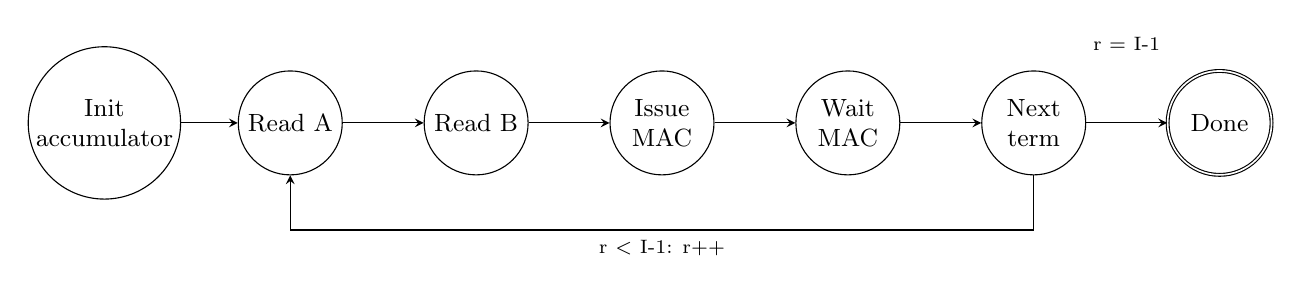
\begin{tikzpicture}[x=0.02cm,y=-0.02cm,>=stealth,every node/.style={font=\small,align=center}]
\node[draw,circle,minimum size=1.32cm,inner sep=1pt] (n0) at (45,85) {Init\\accumulator};
\node[draw,circle,minimum size=1.32cm,inner sep=1pt] (n1) at (163,85) {Read A};
\node[draw,circle,minimum size=1.32cm,inner sep=1pt] (n2) at (281,85) {Read B};
\node[draw,circle,minimum size=1.32cm,inner sep=1pt] (n3) at (399,85) {Issue\\MAC};
\node[draw,circle,minimum size=1.32cm,inner sep=1pt] (n4) at (517,85) {Wait\\MAC};
\node[draw,circle,minimum size=1.32cm,inner sep=1pt] (n5) at (635,85) {Next\\term};
\node[draw,circle,minimum size=1.32cm,inner sep=1pt,double] (n6) at (753,85) {Done};
\draw[->] (n0) -- node[above=8mm,font=\scriptsize]{} (n1);
\draw[->] (n1) -- node[above=8mm,font=\scriptsize]{} (n2);
\draw[->] (n2) -- node[above=8mm,font=\scriptsize]{} (n3);
\draw[->] (n3) -- node[above=8mm,font=\scriptsize]{} (n4);
\draw[->] (n4) -- node[above=8mm,font=\scriptsize]{} (n5);
\draw[->] (n5) -- node[above=8mm,font=\scriptsize]{r = I-1} (n6);
\draw[->] (n5.south) -- (635,153) -- node[below,font=\scriptsize]{r $<$ I-1: r++} (163,153) -- (n1.south);
\end{tikzpicture}}
\end{center}
Initialize the sum, read both numbers, issue one MAC operation, wait for its result and advance $r$. After $I$ terms return the sum. Intermediate sums use more bits than stored outputs to reduce overflow risk.

\newpage
\section*{3\quad Stage 2: Position and read embedding}
\subsection*{Purpose, definitions, input and output}
This stage adds information identifying the position and read of each token.
\begin{itemize}
\item $M$: read slots; $N$: positions per read; $L=MN$: total tokens.
\item $D$: numbers per token, set by the model width.
\item $m$: read index ($0\leq m<M$); $n$: position index ($0\leq n<N$); $j$: feature index ($0\leq j<D$); $t=mN+n$: token index.
\item $P[N,D]$: learned position table; $E[M,D]$: learned read-slot table. They are stored parameters, not calculated from the current input.
\end{itemize}
\textbf{Input:} $e[L,D]$ from Stage 1, plus $P$ and $E$ from parameter memory.

\textbf{Output:} $X^{(0)}[L,D]$, sent to Stage 3. The superscript $(0)$ means before the first encoder layer, not a power. The padding mask is unchanged.

\subsection*{FSM and stage control}
\begin{center}
\resizebox{\textwidth}{!}{%
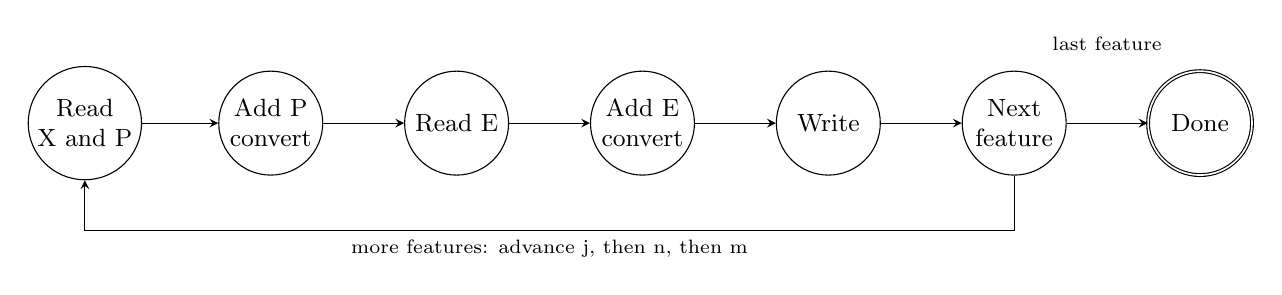
\begin{tikzpicture}[x=0.02cm,y=-0.02cm,>=stealth,every node/.style={font=\small,align=center}]
\node[draw,circle,minimum size=1.32cm,inner sep=1pt] (n0) at (45,85) {Read\\X and P};
\node[draw,circle,minimum size=1.32cm,inner sep=1pt] (n1) at (163,85) {Add P\\convert};
\node[draw,circle,minimum size=1.32cm,inner sep=1pt] (n2) at (281,85) {Read E};
\node[draw,circle,minimum size=1.32cm,inner sep=1pt] (n3) at (399,85) {Add E\\convert};
\node[draw,circle,minimum size=1.32cm,inner sep=1pt] (n4) at (517,85) {Write};
\node[draw,circle,minimum size=1.32cm,inner sep=1pt] (n5) at (635,85) {Next\\feature};
\node[draw,circle,minimum size=1.32cm,inner sep=1pt,double] (n6) at (753,85) {Done};
\draw[->] (n0) -- node[above=8mm,font=\scriptsize]{} (n1);
\draw[->] (n1) -- node[above=8mm,font=\scriptsize]{} (n2);
\draw[->] (n2) -- node[above=8mm,font=\scriptsize]{} (n3);
\draw[->] (n3) -- node[above=8mm,font=\scriptsize]{} (n4);
\draw[->] (n4) -- node[above=8mm,font=\scriptsize]{} (n5);
\draw[->] (n5) -- node[above=8mm,font=\scriptsize]{last feature} (n6);
\draw[->] (n5.south) -- (635,153) -- node[below,font=\scriptsize]{more features: advance j, then n, then m} (45,153) -- (n0.south);
\end{tikzpicture}}
\end{center}
Initialize $m=n=j=0$. The diagram's Read X state reads $e_t[j]$ from working memory. Read its position value, add it, read its read-slot value, add it and write. Convert means rounding and, if necessary, saturation to the stored number format.

Advance $j$ after each finished write. At $j=D-1$, reset $j$ and advance $n$. At $n=N-1$, also reset $n$ and advance $m$. After $MND$ writes, start Stage 3. These are exact integer counters, not quantized feature values.

\subsection*{Math and storage}
\[
a_t[j]=e_t[j]+P[n,j],\qquad X^{(0)}_t[j]=a_t[j]+E[m,j].
\]
$a_t[j]$ is the temporary result after the position addition. Keep the two additions in this order to match Python. The result may replace the old value in the same memory location, but only after that value has been read. Each token still contains $D$ numbers.

\newpage
\section*{4\quad Stage 3: Encoder layers}
\subsection*{Purpose, definitions, input and output}
The encoder lets tokens use information from other tokens, then processes each token through a feed-forward network.
\begin{itemize}
\item $M$: read slots; $N$: positions per read; $L=MN$: tokens; $D$: numbers per token.
\item $K$: number of encoder layers (\texttt{N\_dec} in the configuration); $k=0,\ldots,K-1$ selects the layer.
\item $H$: number of attention heads (\texttt{h} in the configuration). A head uses a group of $d=D/H$ numbers from each query, key and value. $D$ must be divisible by $H$.
\item $t$: token index, $0\leq t<L$. $K,H,D$ are configuration choices, not learned weights.
\item $\LN_1,\LN_2$: the two normalization blocks in a layer. FFN means feed-forward network, defined below.
\end{itemize}
\textbf{Input:} $X^{(0)}[L,D]$ from Stage 2, the stored padding mask $[M,N]$ and trained parameters for all $K$ layers.

\textbf{Output:} $X^{(K)}[L,D]$ for Stage 4. The superscript counts completed layers. Each layer keeps the same number of tokens and numbers per token.

\subsection*{FSM and stage control}
One physical layer is used $K$ times, with different trained parameters for each use.
\begin{center}
\resizebox{\textwidth}{!}{%
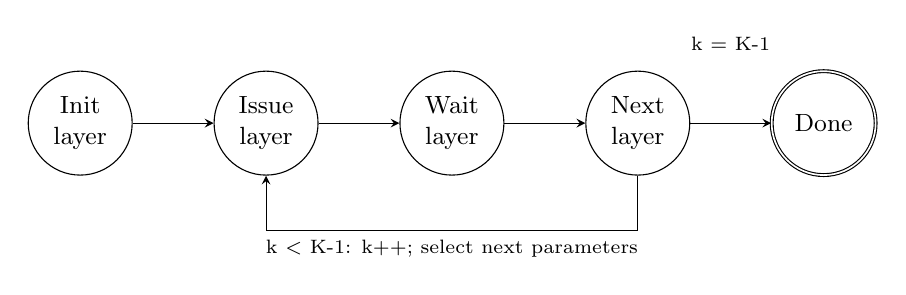
\begin{tikzpicture}[x=0.02cm,y=-0.02cm,>=stealth,every node/.style={font=\small,align=center}]
\node[draw,circle,minimum size=1.32cm,inner sep=1pt] (n0) at (45,85) {Init\\layer};
\node[draw,circle,minimum size=1.32cm,inner sep=1pt] (n1) at (163,85) {Issue\\layer};
\node[draw,circle,minimum size=1.32cm,inner sep=1pt] (n2) at (281,85) {Wait\\layer};
\node[draw,circle,minimum size=1.32cm,inner sep=1pt] (n3) at (399,85) {Next\\layer};
\node[draw,circle,minimum size=1.32cm,inner sep=1pt,double] (n4) at (517,85) {Done};
\draw[->] (n0) -- node[above=8mm,font=\scriptsize]{} (n1);
\draw[->] (n1) -- node[above=8mm,font=\scriptsize]{} (n2);
\draw[->] (n2) -- node[above=8mm,font=\scriptsize]{} (n3);
\draw[->] (n3) -- node[above=8mm,font=\scriptsize]{k = K-1} (n4);
\draw[->] (n3.south) -- (399,153) -- node[below,font=\scriptsize]{k $<$ K-1: k++; select next parameters} (163,153) -- (n1.south);
\end{tikzpicture}}
\end{center}
Initialize $k=0$, select its parameters, start the layer and wait for all output writes. Advance $k$ and repeat. After layer $K-1$, release the result to Stage 4.

\textbf{Inside one layer:}
\begin{center}
\resizebox{\textwidth}{!}{%
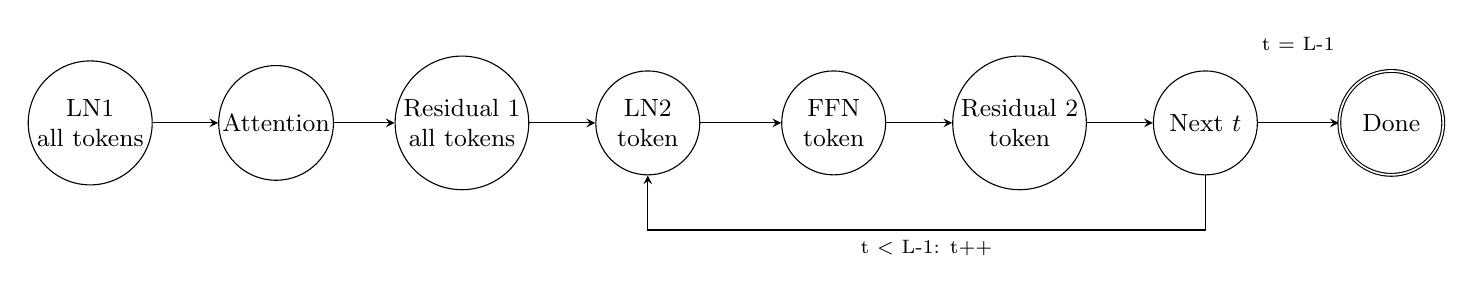
\begin{tikzpicture}[x=0.02cm,y=-0.02cm,>=stealth,every node/.style={font=\small,align=center}]
\node[draw,circle,minimum size=1.32cm,inner sep=1pt] (n0) at (45,85) {LN1\\all tokens};
\node[draw,circle,minimum size=1.32cm,inner sep=1pt] (n1) at (163,85) {Attention};
\node[draw,circle,minimum size=1.32cm,inner sep=1pt] (n2) at (281,85) {Residual 1\\all tokens};
\node[draw,circle,minimum size=1.32cm,inner sep=1pt] (n3) at (399,85) {LN2\\token};
\node[draw,circle,minimum size=1.32cm,inner sep=1pt] (n4) at (517,85) {FFN\\token};
\node[draw,circle,minimum size=1.32cm,inner sep=1pt] (n5) at (635,85) {Residual 2\\token};
\node[draw,circle,minimum size=1.32cm,inner sep=1pt] (n6) at (753,85) {Next $t$};
\node[draw,circle,minimum size=1.32cm,inner sep=1pt,double] (n7) at (871,85) {Done};
\draw[->] (n0) -- node[above=8mm,font=\scriptsize]{} (n1);
\draw[->] (n1) -- node[above=8mm,font=\scriptsize]{} (n2);
\draw[->] (n2) -- node[above=8mm,font=\scriptsize]{} (n3);
\draw[->] (n3) -- node[above=8mm,font=\scriptsize]{} (n4);
\draw[->] (n4) -- node[above=8mm,font=\scriptsize]{} (n5);
\draw[->] (n5) -- node[above=8mm,font=\scriptsize]{} (n6);
\draw[->] (n6) -- node[above=8mm,font=\scriptsize]{t = L-1} (n7);
\draw[->] (n6.south) -- (753,153) -- node[below,font=\scriptsize]{t $<$ L-1: t++} (399,153) -- (n3.south);
\end{tikzpicture}}
\end{center}
Normalize all tokens, finish attention, then add its output to the saved layer input. Next, for each token, run normalization 2, FFN and the second addition. Every block waits for its results to be stored before the dependent block starts.

\subsection*{Math and intermediate values}
Let $X$ be this layer's input:
\[
U=\LN_1(X),\qquad O=\operatorname{Attention}(U),\qquad R=X+O,
\]
\[
T=\LN_2(R),\qquad G=\operatorname{FFN}(T),\qquad X_{\mathrm{next}}=R+G.
\]
$X,U,O,R,T,G$ each contain $L$ tokens with $D$ numbers. $U,T$ are normalized values; $O$ is the attention output; $G$ is the FFN output; $R$ is the first addition's result.
A \textbf{residual addition} adds a block's output to its saved input. Keep $X$ until the first addition and $R$ until the second. Dropout, which randomly removes values during training, is disabled during inference.

\subsection*{Block 1: Normalization 1}
\textbf{Input:} $X_t[D]$. \textbf{Output:} $U_t[D]$, for each token.
For an input token $a$:
\[
\mu=\frac1D\sum_{j=0}^{D-1}a_j,\quad
v=\frac1D\sum_{j=0}^{D-1}(a_j-\mu)^2,\quad
o_j=\gamma_j(a_j-\mu)/\sqrt{v+\epsilon}+\beta_j.
\]
$j$ selects a feature; $\mu$ is the mean; $v$ is the mean squared distance from the mean; $\epsilon=10^{-5}$ prevents division by zero. $\gamma,\beta$ are learned scale and offset values; $o$ is the output. Here $a=X_t$ and $o=U_t$.
\begin{center}
\resizebox{\textwidth}{!}{%
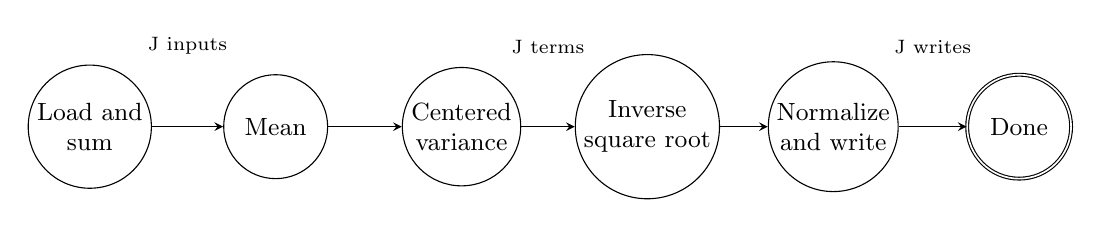
\begin{tikzpicture}[x=0.02cm,y=-0.02cm,>=stealth,every node/.style={font=\small,align=center}]
\node[draw,circle,minimum size=1.32cm,inner sep=1pt] (n0) at (45,85) {Load and\\sum};
\node[draw,circle,minimum size=1.32cm,inner sep=1pt] (n1) at (163,85) {Mean};
\node[draw,circle,minimum size=1.32cm,inner sep=1pt] (n2) at (281,85) {Centered\\variance};
\node[draw,circle,minimum size=1.32cm,inner sep=1pt] (n3) at (399,85) {Inverse\\square root};
\node[draw,circle,minimum size=1.32cm,inner sep=1pt] (n4) at (517,85) {Normalize\\and write};
\node[draw,circle,minimum size=1.32cm,inner sep=1pt,double] (n5) at (635,85) {Done};
\draw[->] (n0) -- node[above=8mm,font=\scriptsize]{J inputs} (n1);
\draw[->] (n1) -- node[above=8mm,font=\scriptsize]{} (n2);
\draw[->] (n2) -- node[above=8mm,font=\scriptsize]{J terms} (n3);
\draw[->] (n3) -- node[above=8mm,font=\scriptsize]{} (n4);
\draw[->] (n4) -- node[above=8mm,font=\scriptsize]{J writes} (n5);
\end{tikzpicture}}
\end{center}
Here $J=D$. Sum the inputs, calculate their mean, calculate variance, calculate $1/\sqrt{v+\epsilon}$, then normalize and write all $D$ outputs. Repeat for all $L$ tokens before attention.

\subsection*{Block 2: Self attention --- input, output and FSM}
\textbf{Input:} $U[L,D]$ and the padding mask. \textbf{Output:} $O[L,D]$.
A \textbf{query} describes what a token looks for; a \textbf{key} is compared with the query; a \textbf{value} supplies the numbers combined using those comparison scores.
\begin{center}
\resizebox{\textwidth}{!}{%
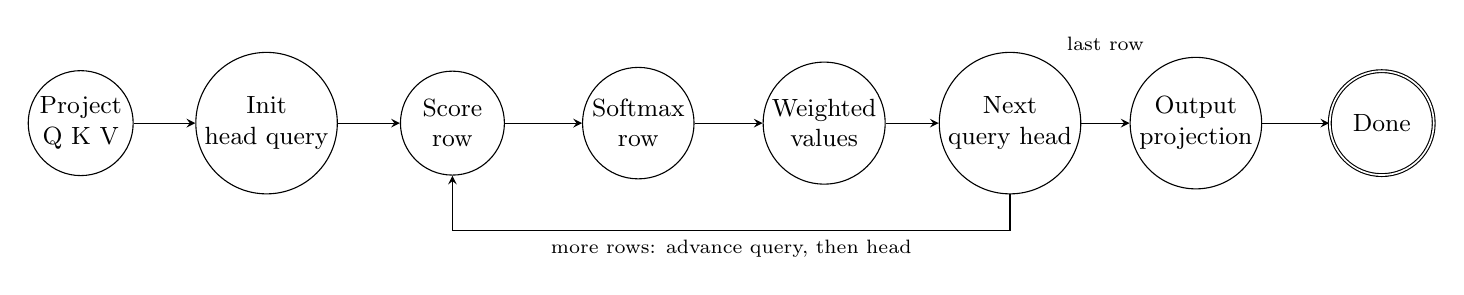
\begin{tikzpicture}[x=0.02cm,y=-0.02cm,>=stealth,every node/.style={font=\small,align=center}]
\node[draw,circle,minimum size=1.32cm,inner sep=1pt] (n0) at (45,85) {Project\\Q K V};
\node[draw,circle,minimum size=1.32cm,inner sep=1pt] (n1) at (163,85) {Init\\head query};
\node[draw,circle,minimum size=1.32cm,inner sep=1pt] (n2) at (281,85) {Score\\row};
\node[draw,circle,minimum size=1.32cm,inner sep=1pt] (n3) at (399,85) {Softmax\\row};
\node[draw,circle,minimum size=1.32cm,inner sep=1pt] (n4) at (517,85) {Weighted\\values};
\node[draw,circle,minimum size=1.32cm,inner sep=1pt] (n5) at (635,85) {Next\\query head};
\node[draw,circle,minimum size=1.32cm,inner sep=1pt] (n6) at (753,85) {Output\\projection};
\node[draw,circle,minimum size=1.32cm,inner sep=1pt,double] (n7) at (871,85) {Done};
\draw[->] (n0) -- node[above=8mm,font=\scriptsize]{} (n1);
\draw[->] (n1) -- node[above=8mm,font=\scriptsize]{} (n2);
\draw[->] (n2) -- node[above=8mm,font=\scriptsize]{} (n3);
\draw[->] (n3) -- node[above=8mm,font=\scriptsize]{} (n4);
\draw[->] (n4) -- node[above=8mm,font=\scriptsize]{} (n5);
\draw[->] (n5) -- node[above=8mm,font=\scriptsize]{last row} (n6);
\draw[->] (n6) -- node[above=8mm,font=\scriptsize]{} (n7);
\draw[->] (n5.south) -- (635,153) -- node[below,font=\scriptsize]{more rows: advance query, then head} (281,153) -- (n2.south);
\end{tikzpicture}}
\end{center}
Calculate all queries, then keys, then values. For one head and query, calculate $L$ scores, convert them to weights using softmax and calculate its $d$ weighted outputs. Advance the query, then the head. After all heads finish, run the output projection. Here $a=0,\ldots,H-1$ selects a head and $i=0,\ldots,L-1$ selects a query token.

\subsubsection*{2a. Query, key and value calculations}
\[
Q=UW_Q^{\mathsf T}+b_Q,\quad
K_{\mathrm{key}}=UW_K^{\mathsf T}+b_K,\quad
V=UW_V^{\mathsf T}+b_V.
\]
$Q,K_{\mathrm{key}},V$ each have shape $[L,D]$. $K_{\mathrm{key}}$ means keys, not the layer count $K$. Each $W$ is a learned $D\times D$ weight table; each $b$ is a learned $D$-number bias. $\mathsf T$ means transpose: weights are arranged to form one weighted sum per output. Use the Stage 1 linear operation, now with $D$ inputs and $D$ outputs.

\subsubsection*{2b. Comparison scores}
For query $i$, head $a$ and key token $j$:
\[
s_j=\frac1{\sqrt d}\sum_{r=0}^{d-1}Q_{i,ad+r}(K_{\mathrm{key}})_{j,ad+r},
\qquad 0\leq j<L.
\]
$s_j$ is the comparison score; $r$ selects a feature within the head; $ad+r$ selects it in the full token.
\begin{center}
\resizebox{\textwidth}{!}{%
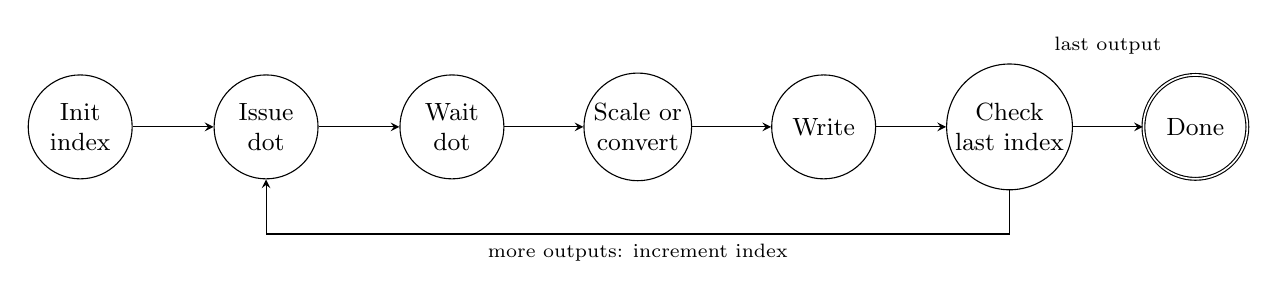
\begin{tikzpicture}[x=0.02cm,y=-0.02cm,>=stealth,every node/.style={font=\small,align=center}]
\node[draw,circle,minimum size=1.32cm,inner sep=1pt] (n0) at (45,85) {Init\\index};
\node[draw,circle,minimum size=1.32cm,inner sep=1pt] (n1) at (163,85) {Issue\\dot};
\node[draw,circle,minimum size=1.32cm,inner sep=1pt] (n2) at (281,85) {Wait\\dot};
\node[draw,circle,minimum size=1.32cm,inner sep=1pt] (n3) at (399,85) {Scale or\\convert};
\node[draw,circle,minimum size=1.32cm,inner sep=1pt] (n4) at (517,85) {Write};
\node[draw,circle,minimum size=1.32cm,inner sep=1pt] (n5) at (635,85) {Check\\last index};
\node[draw,circle,minimum size=1.32cm,inner sep=1pt,double] (n6) at (753,85) {Done};
\draw[->] (n0) -- node[above=8mm,font=\scriptsize]{} (n1);
\draw[->] (n1) -- node[above=8mm,font=\scriptsize]{} (n2);
\draw[->] (n2) -- node[above=8mm,font=\scriptsize]{} (n3);
\draw[->] (n3) -- node[above=8mm,font=\scriptsize]{} (n4);
\draw[->] (n4) -- node[above=8mm,font=\scriptsize]{} (n5);
\draw[->] (n5) -- node[above=8mm,font=\scriptsize]{last output} (n6);
\draw[->] (n5.south) -- (635,153) -- node[below,font=\scriptsize]{more outputs: increment index} (163,153) -- (n1.south);
\end{tikzpicture}}
\end{center}
Request a dot product of $d$ pairs, wait, multiply by the stored constant $1/\sqrt d$, convert the number format and write. Repeat for $L$ keys. A dot product multiplies corresponding numbers and sums the products. Store the entire score row before softmax.

\subsubsection*{2c. Softmax and padding}
Softmax converts the $L$ scores into nonnegative weights whose ideal sum is one:
\[
m_s=\max_j s_j,\quad e_j=\exp(s_j-m_s),\quad
S_{\exp}=\sum_{j=0}^{L-1}e_j,\quad p_j=e_j/S_{\exp}.
\]
$m_s$ is the largest score; $\exp$ is the exponential function; $e_j$ is its result; $S_{\exp}$ is their sum (not the Stage 1 window dimension $S$). Subtracting the maximum limits the exponential's input range.
\begin{center}
\resizebox{\textwidth}{!}{%
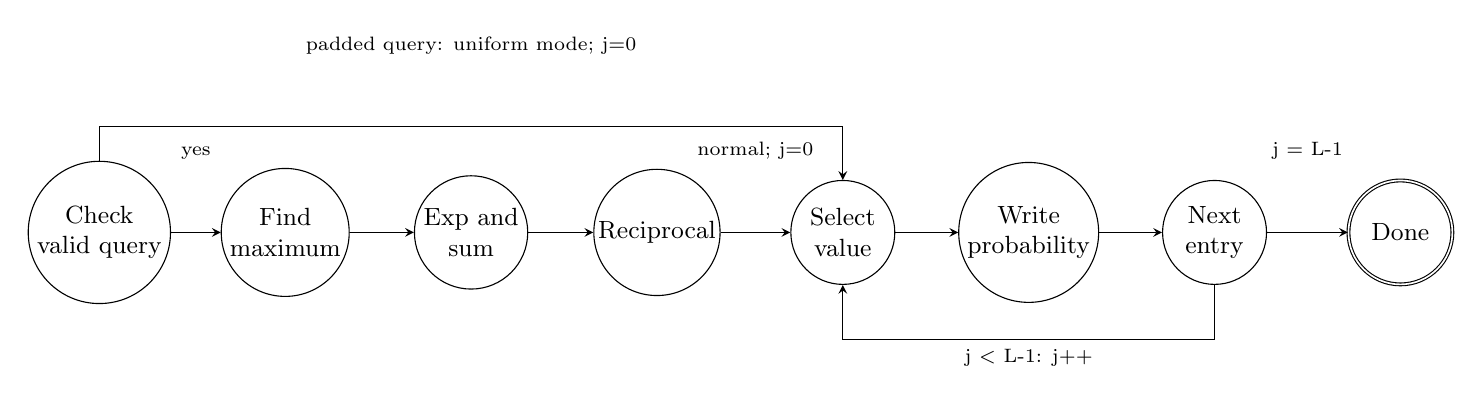
\begin{tikzpicture}[x=0.02cm,y=-0.02cm,>=stealth,every node/.style={font=\small,align=center}]
\node[draw,circle,minimum size=1.32cm,inner sep=1pt] (n0) at (45,85) {Check\\valid query};
\node[draw,circle,minimum size=1.32cm,inner sep=1pt] (n1) at (163,85) {Find\\maximum};
\node[draw,circle,minimum size=1.32cm,inner sep=1pt] (n2) at (281,85) {Exp and\\sum};
\node[draw,circle,minimum size=1.32cm,inner sep=1pt] (n3) at (399,85) {Reciprocal};
\node[draw,circle,minimum size=1.32cm,inner sep=1pt] (n4) at (517,85) {Select\\value};
\node[draw,circle,minimum size=1.32cm,inner sep=1pt] (n5) at (635,85) {Write\\probability};
\node[draw,circle,minimum size=1.32cm,inner sep=1pt] (n6) at (753,85) {Next\\entry};
\node[draw,circle,minimum size=1.32cm,inner sep=1pt,double] (n7) at (871,85) {Done};
\draw[->] (n0) -- node[above=8mm,font=\scriptsize]{yes} (n1);
\draw[->] (n1) -- node[above=8mm,font=\scriptsize]{} (n2);
\draw[->] (n2) -- node[above=8mm,font=\scriptsize]{} (n3);
\draw[->] (n3) -- node[above=8mm,font=\scriptsize]{normal; j=0} (n4);
\draw[->] (n4) -- node[above=8mm,font=\scriptsize]{} (n5);
\draw[->] (n5) -- node[above=8mm,font=\scriptsize]{} (n6);
\draw[->] (n6) -- node[above=8mm,font=\scriptsize]{j = L-1} (n7);
\draw[->] (n6.south) -- (753,153) -- node[below,font=\scriptsize]{j $<$ L-1: j++} (517,153) -- (n4.south);
\draw[->] (n0.north) -- (45,18) -- node[above=8mm,font=\scriptsize]{padded query: uniform mode; j=0} (517,18) -- (n4.north);
\end{tikzpicture}}
\end{center}
For an unpadded query, find the maximum, calculate and sum exponentials, calculate the reciprocal $1/S_{\exp}$, then multiply each $e_j$ by it and write. Reciprocal means one divided by a number. A nonpositive sum reports an error.

The source model masks query rows, not key columns. A padded query gets the same weight $1/L$ for every key. Its FSM skips the exponential calculations and uses the same writer. Unpadded queries can still use padded keys. Preserve this source behavior; changing it needs a separate model decision. The optional static attention mask is excluded from this baseline.

\subsubsection*{2d. Weighted values and output projection}
\[
Z_{i,ad+r}=\sum_{j=0}^{L-1}p_jV_{j,ad+r},\qquad 0\leq r<d.
\]
$Z[L,D]$ stores the results from all heads. Use the score/weighted-value FSM above, now with $L$ terms per dot product and $d$ outputs. Convert and write without the score's extra $1/\sqrt d$ scaling. Keep the weights $p_j$ until all $d$ outputs finish.

Then calculate:
\[
O=ZW_O^{\mathsf T}+b_O.
\]
$W_O[D,D],b_O[D]$ are trained parameters; each output token uses all $D$ numbers of its corresponding $Z$ token.
\begin{center}
\resizebox{\textwidth}{!}{%
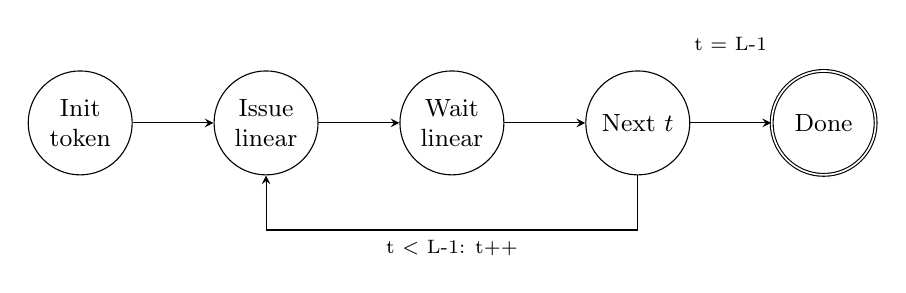
\begin{tikzpicture}[x=0.02cm,y=-0.02cm,>=stealth,every node/.style={font=\small,align=center}]
\node[draw,circle,minimum size=1.32cm,inner sep=1pt] (n0) at (45,85) {Init\\token};
\node[draw,circle,minimum size=1.32cm,inner sep=1pt] (n1) at (163,85) {Issue\\linear};
\node[draw,circle,minimum size=1.32cm,inner sep=1pt] (n2) at (281,85) {Wait\\linear};
\node[draw,circle,minimum size=1.32cm,inner sep=1pt] (n3) at (399,85) {Next $t$};
\node[draw,circle,minimum size=1.32cm,inner sep=1pt,double] (n4) at (517,85) {Done};
\draw[->] (n0) -- node[above=8mm,font=\scriptsize]{} (n1);
\draw[->] (n1) -- node[above=8mm,font=\scriptsize]{} (n2);
\draw[->] (n2) -- node[above=8mm,font=\scriptsize]{} (n3);
\draw[->] (n3) -- node[above=8mm,font=\scriptsize]{t = L-1} (n4);
\draw[->] (n3.south) -- (399,153) -- node[below,font=\scriptsize]{t $<$ L-1: t++} (163,153) -- (n1.south);
\end{tikzpicture}}
\end{center}
Here the linear block has $D$ inputs and $D$ outputs. Start at $t=0$, request a token's calculation, wait for its writes and advance. Finish all $L$ tokens before residual addition 1. Store all Q/K/V tokens, but only one query's scores, exponentials and weights at a time.

\subsection*{Block 3: First residual addition}
\textbf{Inputs:} saved $X[L,D]$ and attention output $O[L,D]$.
\textbf{Output:} $R[L,D]$.
\[
R_t[j]=X_t[j]+O_t[j],\qquad 0\leq t<L,\quad 0\leq j<D.
\]
The saved input is $X$, not normalized $U$.
\begin{center}
\resizebox{\textwidth}{!}{%
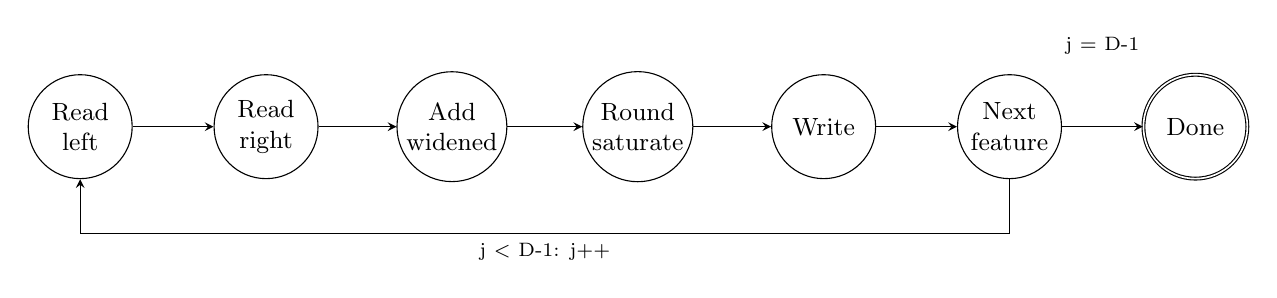
\begin{tikzpicture}[x=0.02cm,y=-0.02cm,>=stealth,every node/.style={font=\small,align=center}]
\node[draw,circle,minimum size=1.32cm,inner sep=1pt] (n0) at (45,85) {Read\\left};
\node[draw,circle,minimum size=1.32cm,inner sep=1pt] (n1) at (163,85) {Read\\right};
\node[draw,circle,minimum size=1.32cm,inner sep=1pt] (n2) at (281,85) {Add\\widened};
\node[draw,circle,minimum size=1.32cm,inner sep=1pt] (n3) at (399,85) {Round\\saturate};
\node[draw,circle,minimum size=1.32cm,inner sep=1pt] (n4) at (517,85) {Write};
\node[draw,circle,minimum size=1.32cm,inner sep=1pt] (n5) at (635,85) {Next\\feature};
\node[draw,circle,minimum size=1.32cm,inner sep=1pt,double] (n6) at (753,85) {Done};
\draw[->] (n0) -- node[above=8mm,font=\scriptsize]{} (n1);
\draw[->] (n1) -- node[above=8mm,font=\scriptsize]{} (n2);
\draw[->] (n2) -- node[above=8mm,font=\scriptsize]{} (n3);
\draw[->] (n3) -- node[above=8mm,font=\scriptsize]{} (n4);
\draw[->] (n4) -- node[above=8mm,font=\scriptsize]{} (n5);
\draw[->] (n5) -- node[above=8mm,font=\scriptsize]{j = D-1} (n6);
\draw[->] (n5.south) -- (635,153) -- node[below,font=\scriptsize]{j $<$ D-1: j++} (45,153) -- (n0.south);
\end{tikzpicture}}
\end{center}
Read both numbers, add using a wider temporary result, round/saturate to the stored format and write. Then advance $j$. Complete $D$ features for all $L$ tokens. Rounding selects a representable number; saturation clips to the format's range. Both operands need the same numerical scale and must be read before overwriting a source location.

\subsection*{Block 4: Normalization 2}
\textbf{Input:} one token $R_t[D]$. \textbf{Output:} $T_t[D]$.
Use the normalization formula and FSM above with $J=D$, but with normalization 2's own learned $\gamma,\beta$. Recalculate mean and variance from $R_t$. Preserve $R_t$ for residual addition 2.

\subsection*{Block 5: Feed-forward network (FFN)}
\textbf{Input:} $T_t[D]$. \textbf{Output:} $G_t[D]$.
The temporary hidden vector has $4D$ numbers; hidden simply means internal to this block.
\begin{center}
\resizebox{\textwidth}{!}{%
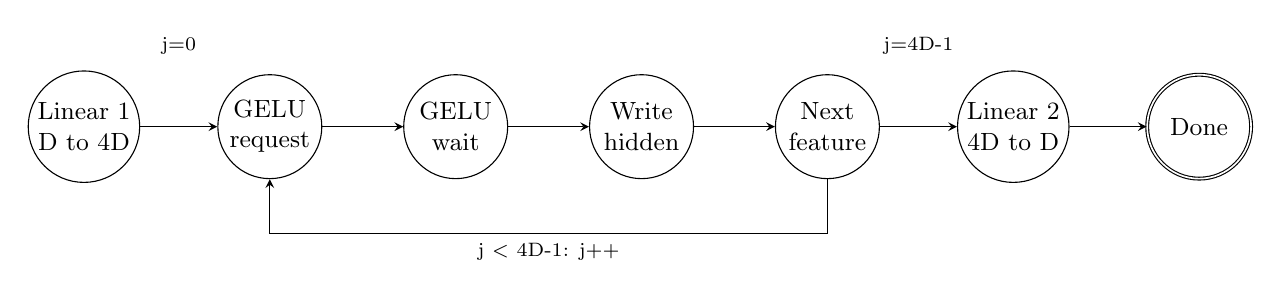
\begin{tikzpicture}[x=0.02cm,y=-0.02cm,>=stealth,every node/.style={font=\small,align=center}]
\node[draw,circle,minimum size=1.32cm,inner sep=1pt] (n0) at (45,85) {Linear 1\\D to 4D};
\node[draw,circle,minimum size=1.32cm,inner sep=1pt] (n1) at (163,85) {GELU\\request};
\node[draw,circle,minimum size=1.32cm,inner sep=1pt] (n2) at (281,85) {GELU\\wait};
\node[draw,circle,minimum size=1.32cm,inner sep=1pt] (n3) at (399,85) {Write\\hidden};
\node[draw,circle,minimum size=1.32cm,inner sep=1pt] (n4) at (517,85) {Next\\feature};
\node[draw,circle,minimum size=1.32cm,inner sep=1pt] (n5) at (635,85) {Linear 2\\4D to D};
\node[draw,circle,minimum size=1.32cm,inner sep=1pt,double] (n6) at (753,85) {Done};
\draw[->] (n0) -- node[above=8mm,font=\scriptsize]{j=0} (n1);
\draw[->] (n1) -- node[above=8mm,font=\scriptsize]{} (n2);
\draw[->] (n2) -- node[above=8mm,font=\scriptsize]{} (n3);
\draw[->] (n3) -- node[above=8mm,font=\scriptsize]{} (n4);
\draw[->] (n4) -- node[above=8mm,font=\scriptsize]{j=4D-1} (n5);
\draw[->] (n5) -- node[above=8mm,font=\scriptsize]{} (n6);
\draw[->] (n4.south) -- (517,153) -- node[below,font=\scriptsize]{j $<$ 4D-1: j++} (163,153) -- (n1.south);
\end{tikzpicture}}
\end{center}
Run linear 1, apply GELU to each of its $4D$ results, then run linear 2. Here $j$ selects a hidden feature, from zero to $4D-1$. Preserve all hidden values until the $D$ outputs finish.
\[
h_t=T_tW_1^{\mathsf T}+b_1,\quad g_t=\GELU(h_t),\quad
G_t=g_tW_2^{\mathsf T}+b_2.
\]
$W_1[4D,D],b_1[4D]$ expand $D$ inputs to $4D$ results $h_t$.
$W_2[D,4D],b_2[D]$ reduce the $4D$ GELU results $g_t$ to $D$ outputs.
GELU is applied separately to each number:
\[
\GELU(x)=x\Phi(x).
\]
$\Phi(x)$ is the probability that a standard normal random variable (mean zero, variance one) is at most $x$. This defines the function; the hardware does not generate random numbers.

\subsection*{Block 6: Second residual addition and completion}
\textbf{Inputs:} saved $R_t[D]$ and FFN output $G_t[D]$.
\textbf{Output:} $X_{\mathrm{next},t}[D]$.
\[
X_{\mathrm{next},t}[j]=R_t[j]+G_t[j].
\]
Use the residual FSM above with left input $R_t$, right input $G_t$ and $D$ outputs. After its writes, process the next token through normalization 2, FFN and residual 2. After all $L$ tokens, start the next layer with its own parameters, or send the final result to Stage 4.

\textbf{Numerical work still required:} GELU, exponential, reciprocal and inverse square root are high-risk numerical blocks. Their fixed-point formats and approximations remain to be validated. Fixed-point means storing numbers with a chosen number of integer and fractional bits.

\newpage
\section*{5\quad Stage 4: Final projection}
\subsection*{Purpose, definitions, input and output}
This stage turns each encoder token into one score.
\begin{itemize}
\item $M$: read slots; $N$: target positions per read; $L=MN$: tokens.
\item $D$: numbers in each encoder token; $K$: number of completed encoder layers.
\item $t=0,\ldots,L-1$: token index; $j=0,\ldots,D-1$: feature index.
\item $w^{final}[D]$: learned final weights; $b^{final}$: learned bias.
\end{itemize}
\textbf{Input:} $X^{(K)}[L,D]$ from Stage 3 and the final weights and bias.

\textbf{Output:} $z[L]$, one logit per token, stored for Stage 5. Equivalently, $z[M,N]$ has one score per read and target position. A logit is a score, not a probability: a positive score favors bit 1 and a negative score favors bit 0.

\subsection*{FSM and stage control}
\begin{center}
\resizebox{\textwidth}{!}{%
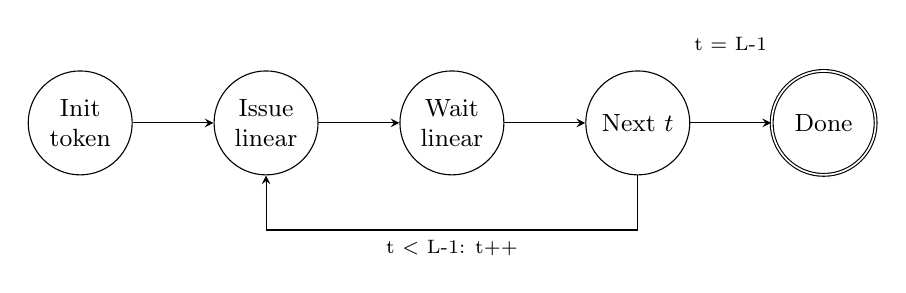
\begin{tikzpicture}[x=0.02cm,y=-0.02cm,>=stealth,every node/.style={font=\small,align=center}]
\node[draw,circle,minimum size=1.32cm,inner sep=1pt] (n0) at (45,85) {Init\\token};
\node[draw,circle,minimum size=1.32cm,inner sep=1pt] (n1) at (163,85) {Issue\\linear};
\node[draw,circle,minimum size=1.32cm,inner sep=1pt] (n2) at (281,85) {Wait\\linear};
\node[draw,circle,minimum size=1.32cm,inner sep=1pt] (n3) at (399,85) {Next $t$};
\node[draw,circle,minimum size=1.32cm,inner sep=1pt,double] (n4) at (517,85) {Done};
\draw[->] (n0) -- node[above=8mm,font=\scriptsize]{} (n1);
\draw[->] (n1) -- node[above=8mm,font=\scriptsize]{} (n2);
\draw[->] (n2) -- node[above=8mm,font=\scriptsize]{} (n3);
\draw[->] (n3) -- node[above=8mm,font=\scriptsize]{t = L-1} (n4);
\draw[->] (n3.south) -- (399,153) -- node[below,font=\scriptsize]{t $<$ L-1: t++} (163,153) -- (n1.south);
\end{tikzpicture}}
\end{center}
Set $t=0$. Request the linear calculation with $D$ inputs and one output. Wait for the result to be converted and stored, then advance $t$. There is no second write by this controller: the linear block already performs it. Start Stage 5 only after all $L$ logits are stored.

\subsection*{Math and internal linear block}
\[
z_t=b^{final}+\sum_{j=0}^{D-1}w^{final}_jX^{(K)}_t[j].
\]
Read the bias, multiply each input by its weight and add all $D$ products to the bias. Then round and, if necessary, clip to the representable range before writing.
\begin{center}
\resizebox{\textwidth}{!}{%
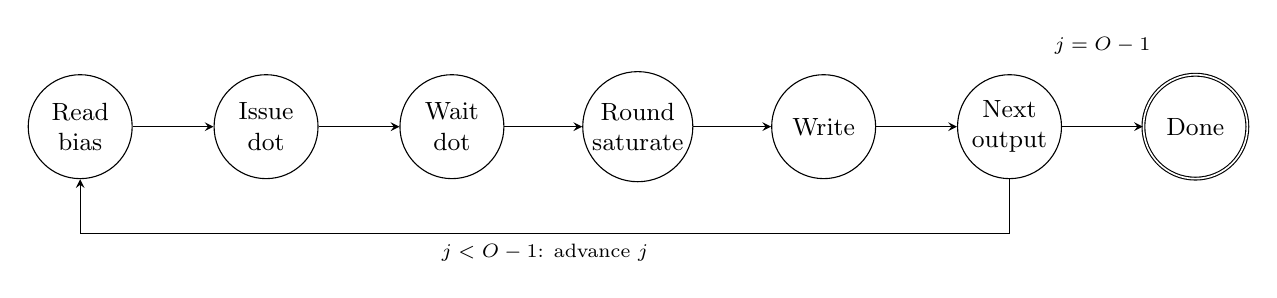
\begin{tikzpicture}[x=0.02cm,y=-0.02cm,>=stealth,every node/.style={font=\small,align=center}]
\node[draw,circle,minimum size=1.32cm,inner sep=1pt] (n0) at (45,85) {Read\\bias};
\node[draw,circle,minimum size=1.32cm,inner sep=1pt] (n1) at (163,85) {Issue\\dot};
\node[draw,circle,minimum size=1.32cm,inner sep=1pt] (n2) at (281,85) {Wait\\dot};
\node[draw,circle,minimum size=1.32cm,inner sep=1pt] (n3) at (399,85) {Round\\saturate};
\node[draw,circle,minimum size=1.32cm,inner sep=1pt] (n4) at (517,85) {Write};
\node[draw,circle,minimum size=1.32cm,inner sep=1pt] (n5) at (635,85) {Next\\output};
\node[draw,circle,minimum size=1.32cm,inner sep=1pt,double] (n6) at (753,85) {Done};
\draw[->] (n0) -- node[above=8mm,font=\scriptsize]{} (n1);
\draw[->] (n1) -- node[above=8mm,font=\scriptsize]{} (n2);
\draw[->] (n2) -- node[above=8mm,font=\scriptsize]{} (n3);
\draw[->] (n3) -- node[above=8mm,font=\scriptsize]{} (n4);
\draw[->] (n4) -- node[above=8mm,font=\scriptsize]{} (n5);
\draw[->] (n5) -- node[above=8mm,font=\scriptsize]{$j = O-1$} (n6);
\draw[->] (n5.south) -- (635,153) -- node[below,font=\scriptsize]{$j < O-1$: advance $j$} (45,153) -- (n0.south);
\end{tikzpicture}}
\end{center}
In this internal FSM $I=D$ is the input count and $O=1$ is the output count. Its output index $j$ therefore stays at zero; it is not the summation index in the equation above. No sigmoid (a function converting a logit into a probability) is applied here.

\newpage
\section*{6\quad Stage 5: Read aggregation}
\subsection*{Purpose, definitions, input and output}
Aggregation means combining the different reads' scores into one score per target position.
\begin{itemize}
\item $M$: read slots; $N$: target positions per read; $L=MN$: input scores.
\item $m=0,\ldots,M-1$: read index; $n=0,\ldots,N-1$: position index.
\item $z_{mN+n}$: Stage 4 logit for read $m$, position $n$.
\item $p^{mask}_{m,n}$: padding flag, one for padding and zero for a real position.
\item $v_{m,n}=1-p^{mask}_{m,n}$: one exactly when read $m$ contributes at position $n$.
\item $C_n=\sum_{m=0}^{M-1}v_{m,n}$: number of valid reads contributing to this specific position $n$.
\end{itemize}
\textbf{Input:} all $L$ logits from Stage 4 and the stored padding mask $[M,N]$.

\textbf{Output:} $N$ logits for a valid frame, one per target bit position. If any position has no valid read, discard the whole frame and report an error instead of transmitting logits.

\subsection*{FSM and stage control}
\begin{center}
\resizebox{\textwidth}{!}{%
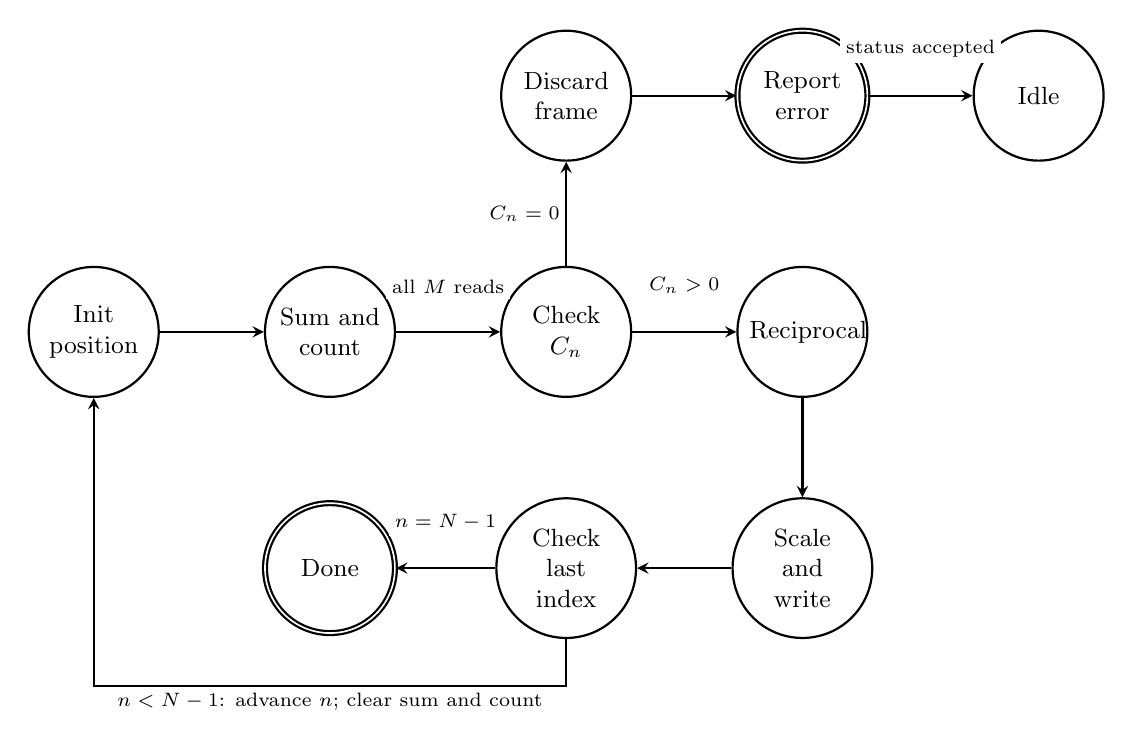
\begin{tikzpicture}[>=stealth,thick,
every node/.style={font=\small,align=center},
st/.style={draw,circle,minimum size=1.65cm,text width=1.35cm,inner sep=1pt},
lab/.style={font=\scriptsize,fill=white,inner sep=2pt}]
\node[st] (init) at (0,0) {Init\\position};
\node[st] (scan) at (3,0) {Sum and\\count};
\node[st] (check) at (6,0) {Check\\$C_n$};
\node[st] (recip) at (9,0) {Reciprocal};
\node[st] (write) at (9,-3) {Scale\\and write};
\node[st] (next) at (6,-3) {Check\\last index};
\node[st,double] (done) at (3,-3) {Done};
\node[st] (drop) at (6,3) {Discard\\frame};
\node[st,double] (error) at (9,3) {Report\\error};
\node[st] (idle) at (12,3) {Idle};
\draw[->] (init)--(scan);
\draw[->] (scan)--node[lab,above=4mm]{all $M$ reads}(check);
\draw[->] (check)--node[lab,above=4mm]{$C_n>0$}(recip);
\draw[->] (recip)--(write);
\draw[->] (write)--(next);
\draw[->] (next)--node[lab,above=4mm]{$n=N-1$}(done);
\draw[->] (next.south)--(6,-4.5)--node[lab,below]{$n<N-1$: advance $n$; clear sum and count}(0,-4.5)--(init.south);
\draw[->] (check)--node[lab,left]{$C_n=0$}(drop);
\draw[->] (drop)--(error);
\draw[->] (error)--node[lab,above=4mm]{status accepted}(idle);
\end{tikzpicture}}
\end{center}
Start with $n=0$. Init position clears $S_n$, $C_n$ and read index $m$. Sum and count scans all $M$ reads: when a position is unpadded, add its logit to $S_n$ and increment $C_n$; otherwise skip both operations. Advance $m$ only after that read's contribution is processed.

If $C_n>0$, calculate $1/C_n$, multiply the sum by it and store the result. After the write finishes, advance to the next position and clear both sum and count. The denominator and reciprocal are calculated separately for every position, not once per frame.

This same rule applies for $M=1$: an unpadded position copies its logit because $C_n=1$; a padded position has $C_n=0$ and takes the error path. There is no mask-ignoring copy branch.

\subsection*{Math}
\[
C_n=\sum_{m=0}^{M-1}(1-p^{mask}_{m,n}),\qquad
S_n=\sum_{m=0}^{M-1}(1-p^{mask}_{m,n})z_{mN+n},
\]
\[
\mathrm{logit}_n=\frac{S_n}{C_n},\qquad C_n>0.
\]
The same validity flag controls both the sum and the count. A partially padded read contributes to both at each unpadded position, and to neither at its padded positions. $S_n$ is a score sum, not the Stage 1 window dimension $S$.

\textbf{Reference-model change:} this is the corrected architecture rule, not the current Python averaging rule. The Python reference must be updated to use per-position counts and the same empty-position error policy before hardware comparison. This document change does not modify the Python implementation.

\subsection*{Zero-count recovery: discard the frame, no reset}
If any $C_n=0$:
\begin{enumerate}[leftmargin=*]
\item Do not request a reciprocal or perform division. Stop calculating further positions.
\item Wait for any already accepted memory operation to finish. Mark the frame's output buffer invalid, including scores already stored for earlier positions. Erasing the stored numbers is unnecessary.
\item Transmit no logits for this frame and do not generate substitute zeros or a success status. Keep output-valid low. Output transfer is permitted only after Stage 5 successfully finishes every position, so no partial frame has been sent.
\item Report \texttt{EMPTY\_POSITION} with the failed position index $n$. Hold the error status and index unchanged until the receiver accepts them. Do not accept another frame while this status is pending.
\item After status acceptance, clear the frame counters and temporary control state and return to idle. Keep trained parameters available. Accept the next frame without a hard reset.
\end{enumerate}
This is a recoverable input-data error, not a fatal hardware fault. If the receiver delays accepting the error status, the ASIC waits in Report error; it does not permanently halt.

\subsection*{Output transfer and frame completion}
Done means every position has a valid stored result. Only then may the frame controller start output transfer. Hold each logit until the receiver accepts it, then advance. Report successful frame completion after all $N$ transfers. If a binary decision is needed afterwards, choose 1 for a positive logit and 0 otherwise.

\newpage
\section*{7\quad Shared implementation and review decisions}
\subsection*{Shared resources and control}
\begin{itemize}
\item \textbf{Dot engine:} initialize bias or zero; read A; read B; issue/wait multiply--accumulate; advance term; return a widened sum. Linear control repeats this for output features and owns rounding, saturation and writes.
\item \textbf{Storage:} parameter memory; X/residual, U, Q/K/V, Z and attention-output banks; token and $4D$ FFN scratch; three length-L row buffers; mask and logit buffers. These are logical banks; SRAM mapping and capacity require the selected dimensions and technology.
\item \textbf{Transactions:} commands and responses use ready/valid with one outstanding operation per engine. Hold payloads stable during stalls. Advance counters only on accepted work; report completion only after committed writes. Fatal hardware errors stop new work, drain accepted transactions and require reset before retry. Stage 5's empty-position error discards only the current frame and returns to idle after error-status acceptance; it does not require reset.
\end{itemize}

\subsection*{Numerical validation and review decisions}
GELU, exponential, reciprocal and inverse square root retain defined request/response interfaces; their implementations and fixed-point formats remain to be selected. Use widened reductions and explicit conversion points. Compare floating-point and bit-accurate intermediate results, record saturation/overflow, then require RTL to match the bit-accurate model. Acceptance must include decoding error rates, not only local arithmetic error.

\textbf{Requested review:} confirm the sequential architecture and model/checkpoint; query masking and padding policy; target memory/clock/throughput constraints; and numerical acceptance criteria. These decisions precede arithmetic-format freeze and integrated RTL implementation.

{\footnotesize Software basis: BCJRFormer, \texttt{bcjrformer.py} and \texttt{modules.py}, repository revision \texttt{c7cf84e218730f4583e79af6dd876b04384d33f5}.}
\end{document}
